\chapter{Introduction}
\labch{intro}

\section{Context}
In the field of material science, Plastics have been booming since the late 1950s\cite{geyer2017production}.It's a problem for ecosystems, on one hand, by the means of production as 90\% of plastics come from fossil fuels. On other hand,because of its widespread presence in ecosystems gradually degraded into microplastics and nanoplastics. Moreover only 9\% of plastics is recycled and 12\% is incinerated almost all other waste is lost in nature\cite{natureeditorial}.

% \begin{marginfigure}
%     %\centering
%     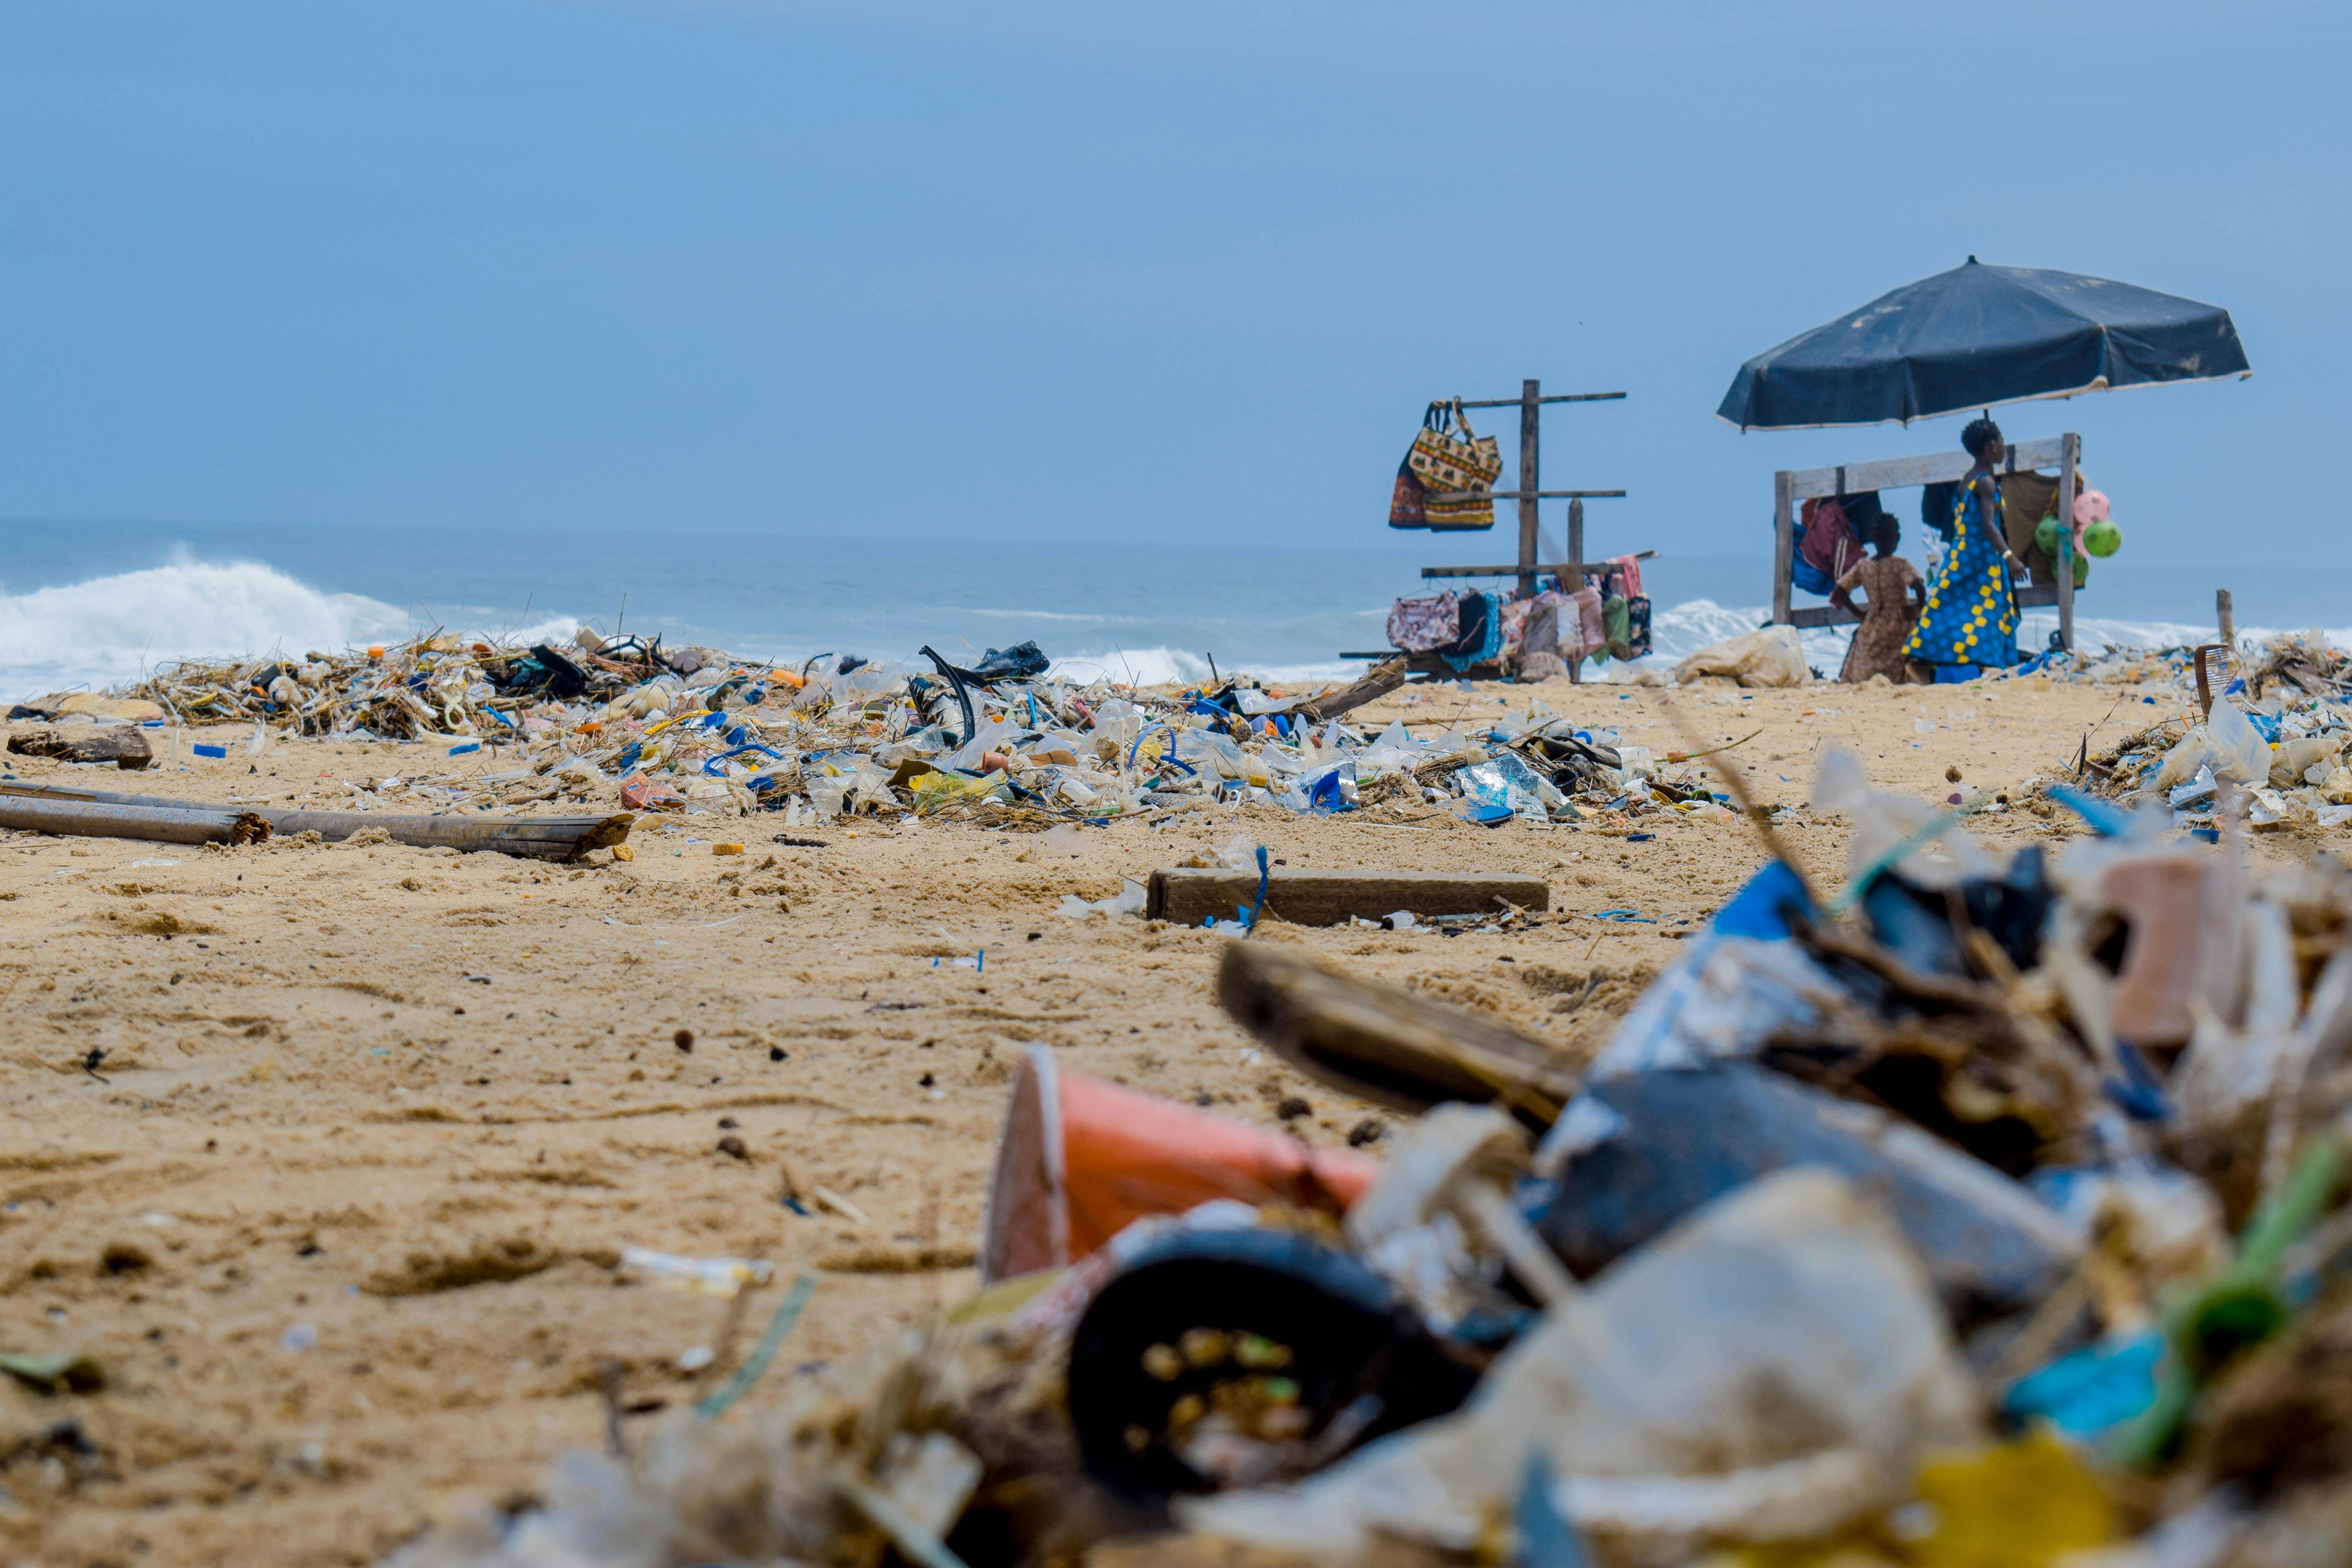
\includegraphics{images/plastic-waste.png}
%     \caption{Plastics pollution on a beach}
%     \label{fig:plastics}
% \end{marginfigure}

\begin{marginfigure}[-5.5cm]
	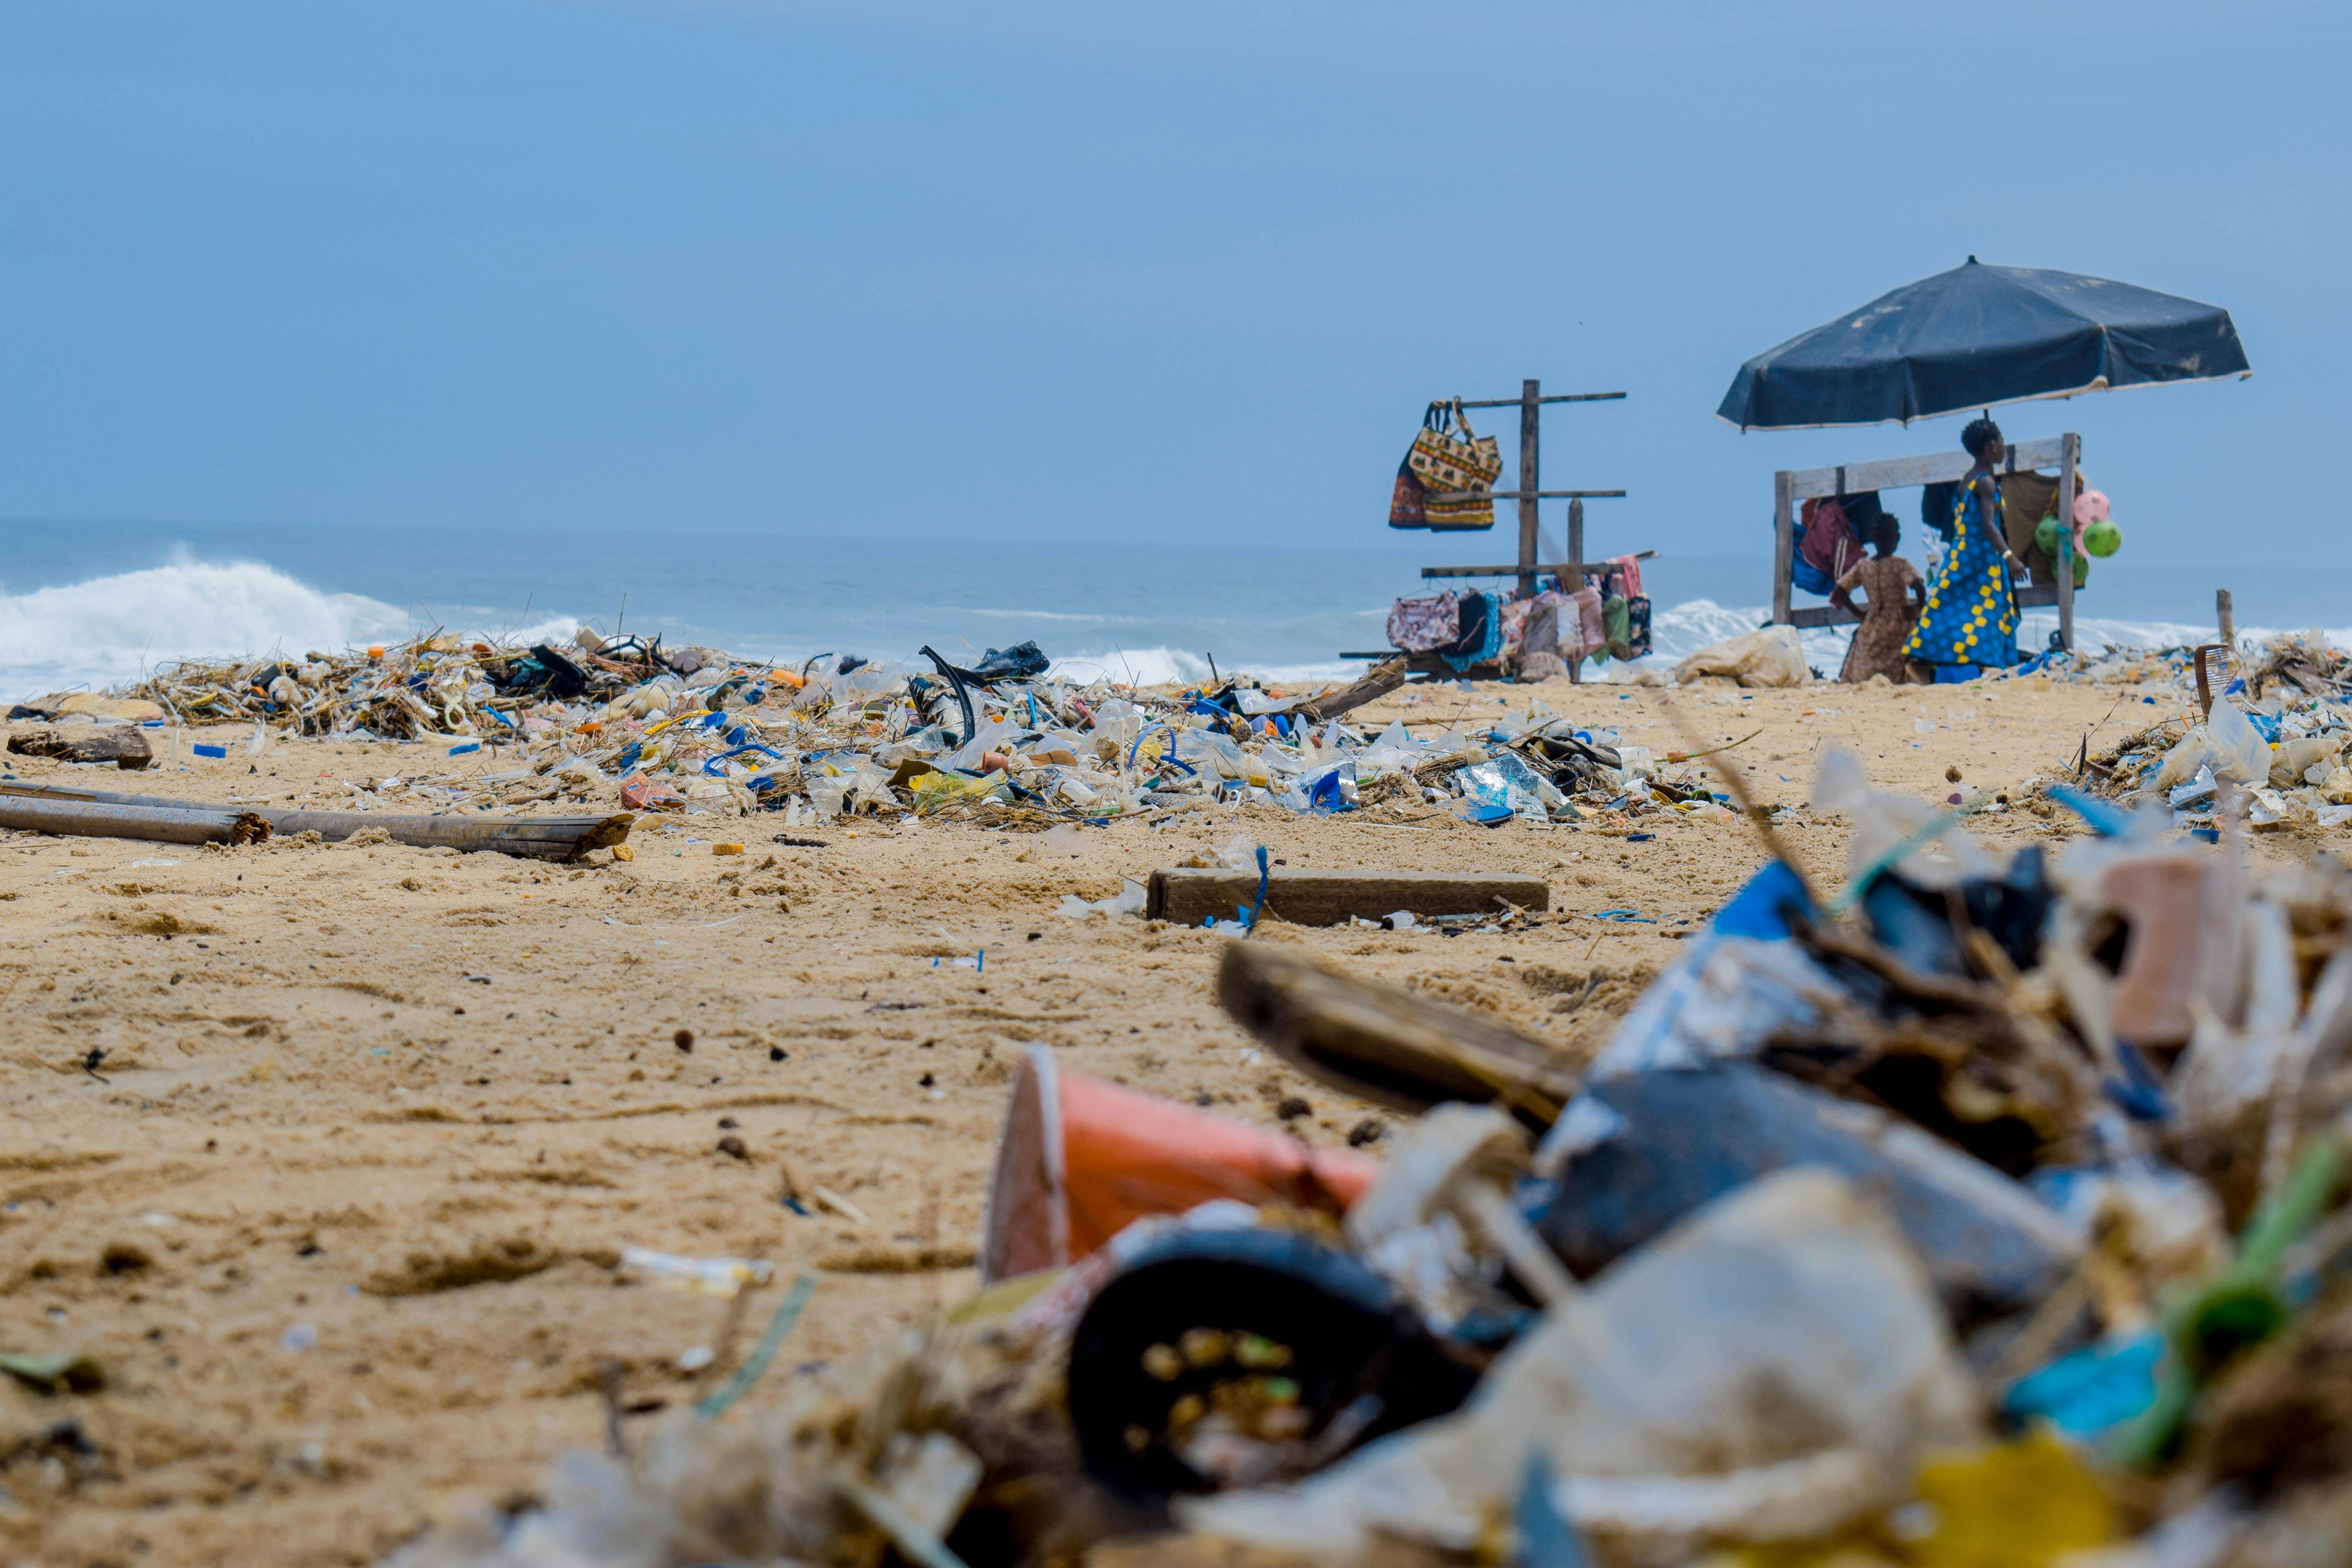
\includegraphics{images/plastic-waste.png}
	\caption[The Mona Lisa]{The Mona Lisa.\\ 
	\url{https://commons.wikimedia.org/wiki/File:Mona_Lisa,_by_Leonardo_da_Vinci,_from_C2RMF_retouched.jpg}}
	\labfig{marginmonalisa}
\end{marginfigure}

\marginnote{
    \centering
    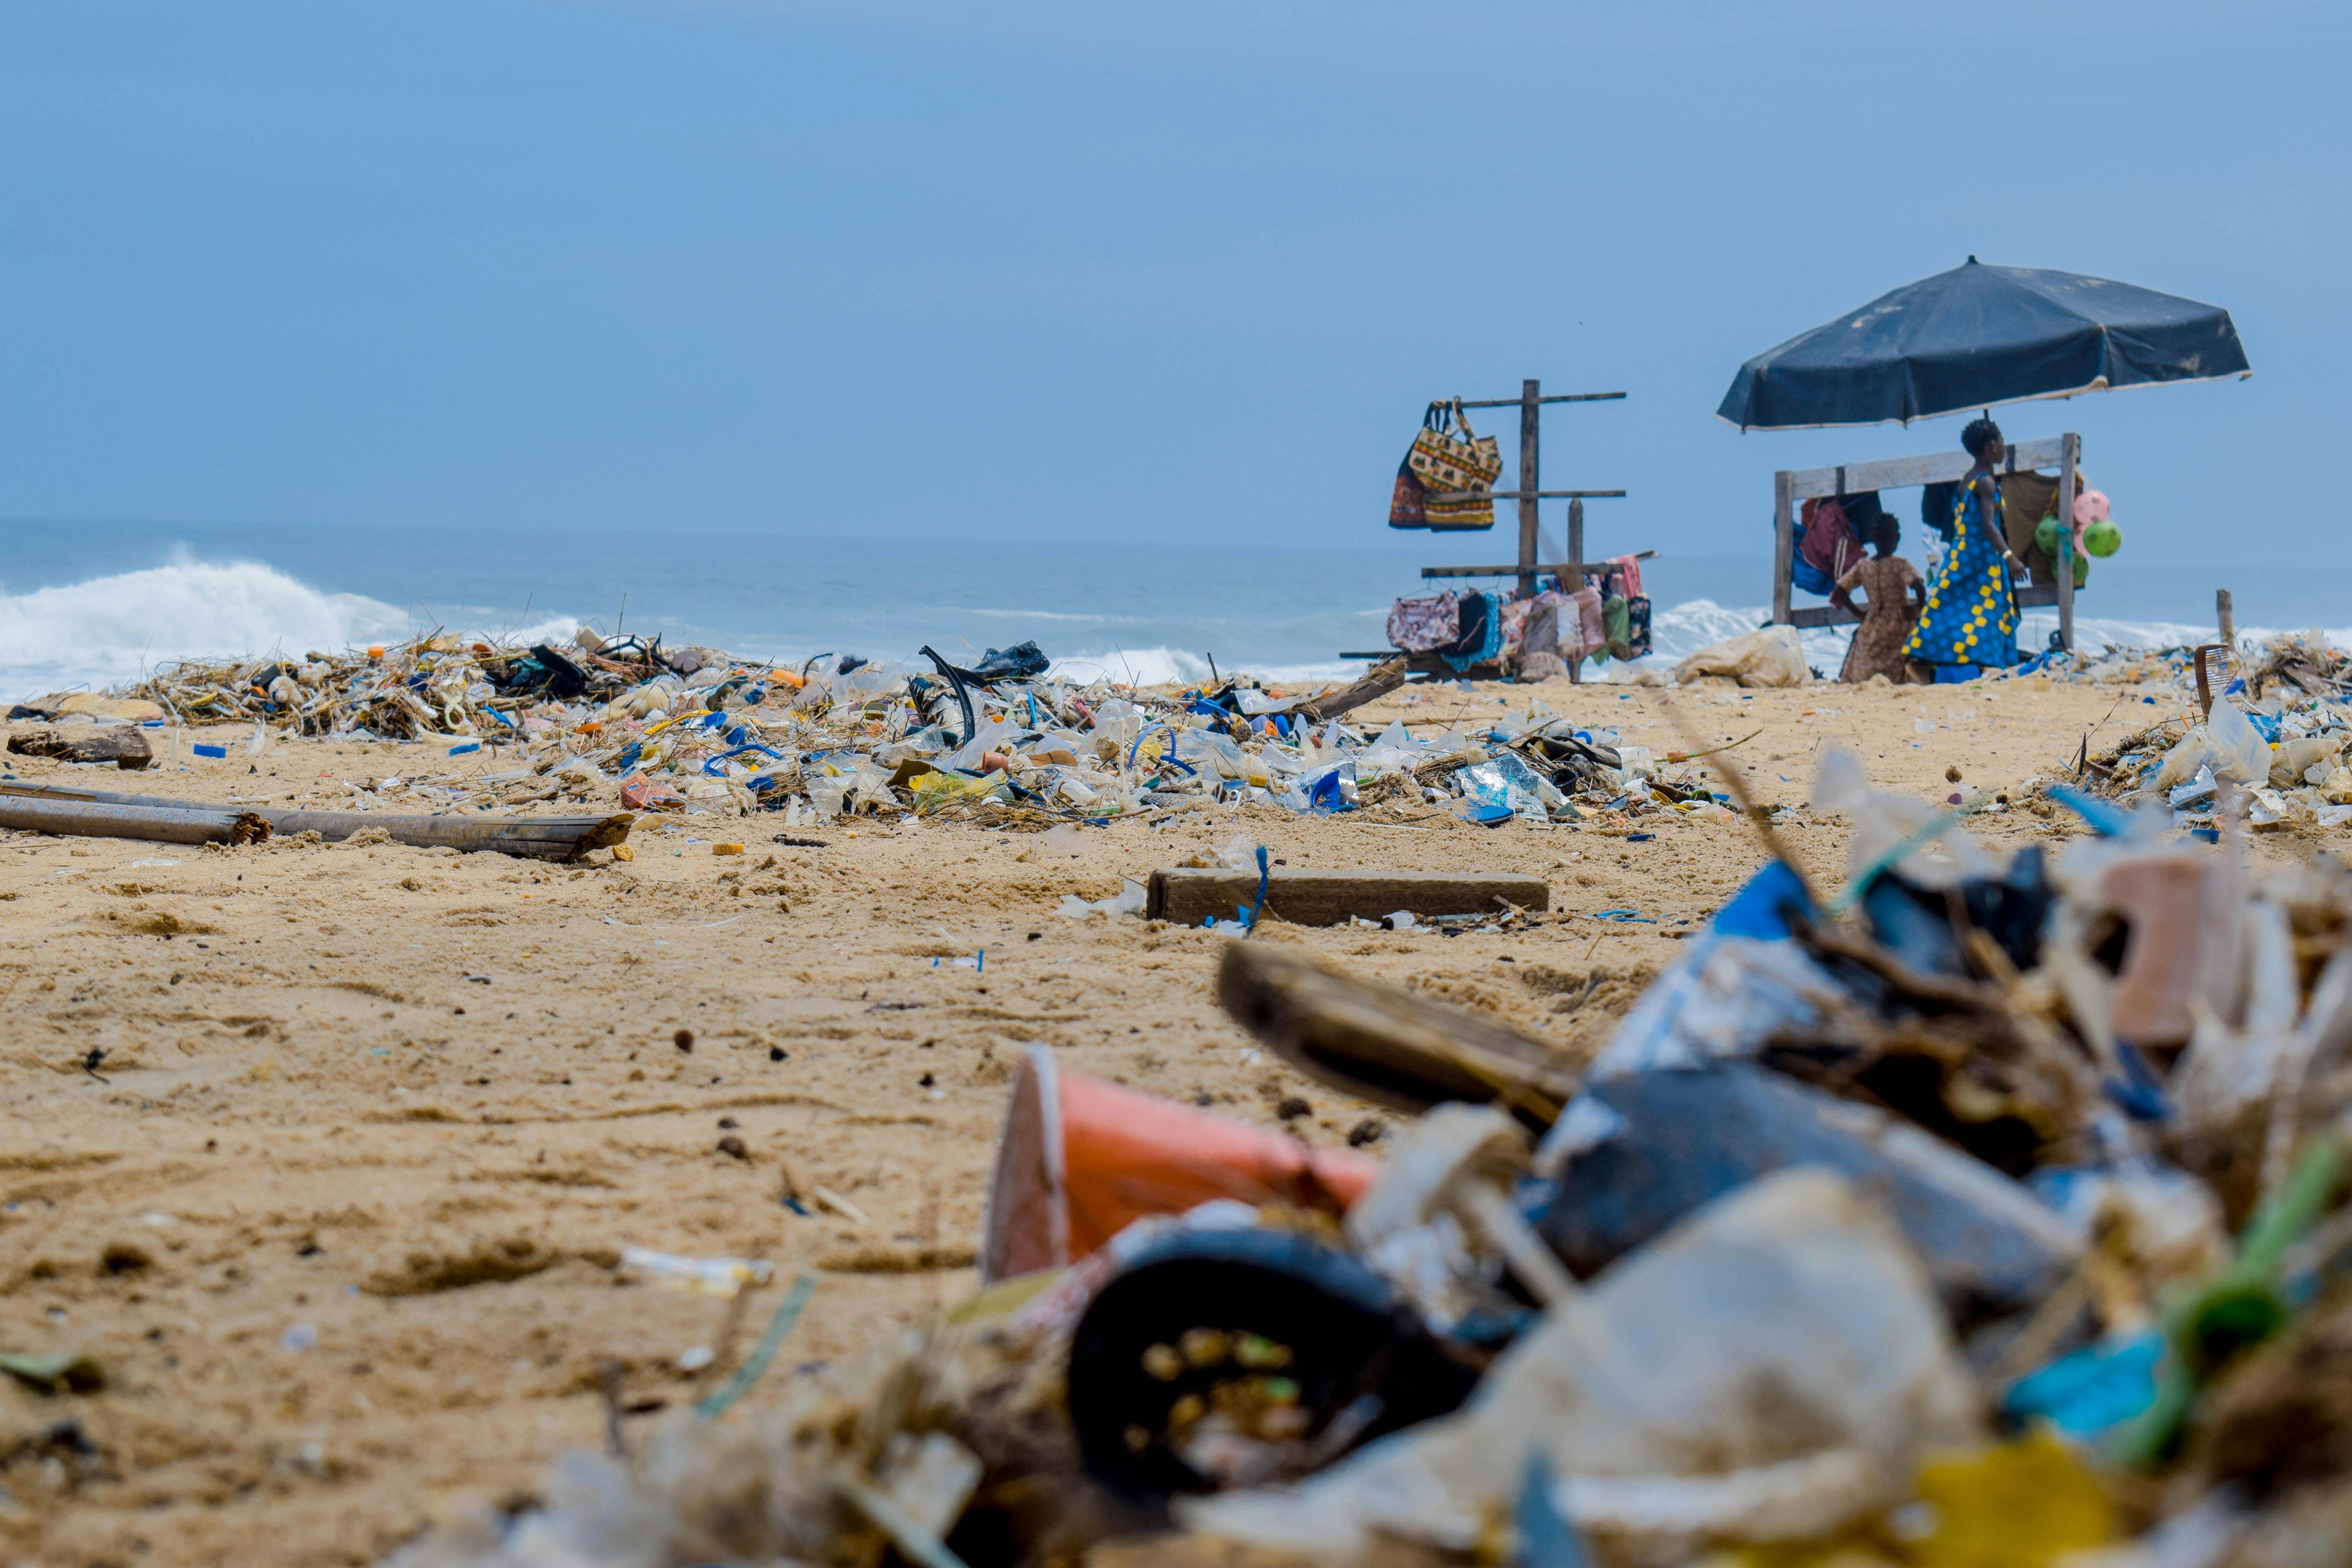
\includegraphics{images/plastic-waste.png}
    \captionof{figure}{Plastics pollution on a beach}
    \label{fig:taele2015maestoso}
}


With plastics, we have a material that our environments can't dissolve and similarly as a a living organism that create it creates an imbalance. Since we have create materials that are "invincible" for the environment,  that environments can't gets rid of, or can't use we've created materials that pollute nature once they're out there.

Moreover we we're moving towards a problem of raw materials in general, independently of plastics. this raises other issues of recycling, delocalization of resources, and the energy needed to extract them from the environment.

That is why, some researcher and designer or other indistrual actor, works on the fabrication of new kind of materials that are biobased.
 
These biosourced materials, which we call biomaterials, have the particularity of being co-created (and sometimes even co-designed) with living organisms. As they are organic materials, this makes them eco-responsible for the environment. 

To makes this kind of biomaterials, it is necessary to understand the living organisms from which it is derived. In order to build machine like controlled environment systems, that reproduces the best growing conditions for our biomaterials.

\section{Approach}
This thesis studies the development and use of biomaterials and the manufacture of a machine tool for biomaterial production.
That is why The areas concerned include biological fermentantion, IOT and sensors, mechanical electronics, and mushroom growth theory. 

Biology is very interesting to make material. In one hand you design new way to create raw materials and be sure that the new materials you create is non toxics for the environment. In other hand, because of the nature of your materials, instead of just creating raw materials you may grow directly concept. 

In both cases, the manufacture of specific controlled environment systems adapted to the biomaterials in question is essential. 
In order to sometimes better understand the growth parameters, optimize biomaterial production, divert or constrain the shape or the way biomaterial grows. 

Furthermore, this thesis also studies the effectiveness and benefits of post-treatment, which may or may not need to be carried out on certain biomaterials 

the general approach is as follows: 

\begin{figure}[h]
    \centering
    \includegraphics{images/diag_approche.png}
    \caption{General approach overview}
    \label{fig:IS_demo}
\end{figure}


\section{Field of Research}

This research is situated at the intersection of biomaterial science, biological growth processes, and environmental control technologies. Specifically, 
it explores the potential of soft biomaterials such as SCOBY (Symbiotic Culture of Bacteria and Yeast) and mycelium biocomposite, two promising alternatives 
for sustainable material production. 

\paragraph[short]{Biomaterial science} 
Biomaterial science forms the foundation of this research by investigating the properties, applications, and fabrication processes of materials derived from living organisms. 
The study of SCOBY mycelium-based biocomposites is still relatively new, yet early research suggests their high potential for applications in various sectors, including fashion\cite{amobonye2023fungal}, architecture\cite{ghazvinian2019mycelium}, and packaging\cite{abhijith2018sustainable}, where ecological impacts are a growing concern. And as a substitute for certain materials currently derived from fossil resources\cite{jang2017bacterial}.

One of the core aspects of this research is the investigation of the biological growth processes that govern the development of these materials. SCOBY, for instance, grows through a fermentation process where bacteria and yeast work together in a chain reaction where bacteria produce cellulose. Mycelium, on the other hand, forms a dense network of fungal hyphae, which can be molded into various shapes and solid structures. Understanding and optimizing the growth parameters—such as temperature, humidity, and nutrient supply—is essential for ensuring the consistency and quality of the biomaterials produced.

\paragraph[short]{Environmental
control technologies}
To achieve optimal growth conditions, this research integrates IoT-based sensors for real-time monitoring and control of environmental factors within bioreactors. 
The sensors pair with actuator, including temperature, pH, and moisture sensors, provides precise feedback, allowing for the automation of the growth process. 
automation of the growth process. System automation also opens the door to the field of embedded systems and electronics research. 

In the field of plant sciece controlled environment systems, like Phytotron are use to recreate climates to studies plants behavior under experimental conditions.
Unlike Phytotron, the role of the bioreactor is not only to recreate optimal growth conditions, but above all to create specific environmental paramenter or special constrain that allowing the bioreactor to amplify unnatural behavior in order to induce new properties on the biomaterial.  This capability allows for greater customization and the exploration of material innovation, as bioreactors can be programmed to create tailored conditions that go beyond natural biological environments.
 

\paragraph[short]{Low-technologies} 
This thesis also draws inspiration from the philosophy of low-technologies.
Low-technologies offer an alternative to high-tech industrial processes by focusing on accessible, repairable, and sustainable solutions. 
This approach not only reduces environmental impacts but also opens up the possibility for decentralized, small-scale production systems that are adaptable to different geographic and climatic conditions. 
Biomaterials meet this definition, and can be include in lager systems to recycled organic waste as illustration. the low-technologies allready use mycelium biocomposite in in building construction. 

whether it's in the use of biomaterials or in machine design. \textbf{design} is also part of the field of research. particularly in the creation of new imaginary worlds that allow us to glimpse new aesthetics that can influence the way we think about matter. 



\section{Contributions}

The contributions to the field mainly focus on what needs this type of material to be grown and how to optimize it.
It focus on two different types of material. Mycelium and S.C.O.B.Y and their respective bioreactor types. 

The projects focus on the production and use of biomaterials and the manufacture of machines to optimize and automate their development, but also to try to disrupt the natural means of growth or co-design with nature to create new uses or forms for biomaterials thanks to the bioreactor. in ways that go beyond the simple production of raw materials.

The goal was also to develop a methodology to understand and build machine tools in order to develop an approach that can be generalized to other biomaterials.
The Machine also aim to be ergonomic and useful for the final user. Because all this type of machine might be build simply by just using a box and some kind of actuator, the projet aim to show that understand deeply the formation of the biomaterial is an added value if we want to be able to divert the living to make more than raw material or a hight tech greenhouse. 
